%%% start preambling . . .  %%%
\documentclass{article}

% required 
\usepackage{amsmath}
\usepackage{natbib}
\usepackage{xr-hyper}
\usepackage{hyperref}
\externaldocument[manuscript-]{manuscript}
\usepackage{booktabs,siunitx}
\usepackage{Sweave}
\usepackage{graphicx}
\usepackage{lipsum}                     % Dummytext % https://tex.stackexchange.com/questions/9796/how-to-add-todo-notes
\usepackage{xargs}                      % Use more than one optional parameter in a new commands
\usepackage[pdftex,dvipsnames]{xcolor}  % Coloured text etc.

\usepackage[colorinlistoftodos,prependcaption,textsize=tiny]{todonotes}
\newcommandx{\unsure}[2][1=]{\todo[linecolor=red,backgroundcolor=red!25,bordercolor=red,#1]{#2}}
\newcommandx{\change}[2][1=]{\todo[linecolor=blue,backgroundcolor=blue!25,bordercolor=blue,#1]{#2}}
\newcommandx{\info}[2][1=]{\todo[linecolor=OliveGreen,backgroundcolor=OliveGreen!25,bordercolor=OliveGreen,#1]{#2}}
\newcommandx{\improvement}[2][1=]{\todo[linecolor=Plum,backgroundcolor=Plum!25,bordercolor=Plum,#1]{#2}}
\newcommandx{\thiswillnotshow}[2][1=]{\todo[disable,#1]{#2}}


% https://tex.stackexchange.com/questions/60209/how-to-add-an-extra-level-of-sections-with-headings-below-subsubsection
\usepackage{titlesec}
\setcounter{secnumdepth}{4}

\titleformat{\paragraph}
{\normalfont\normalsize\bfseries}{\theparagraph}{1em}{}
\titlespacing*{\paragraph}
{0pt}{3.25ex plus 1ex minus .2ex}{1.5ex plus .2ex}



% recommended! Uncomment the below line and change the path for your computer!
 
%put your figures in one place! Also, note that here 'figures' is the folder and 'demoFig' is what each 
% figure produced will be titled plus its number or label (e.g., demoFig-nqpbetter.pdf')

% make your captioning look better
\usepackage[small]{caption}
\setlength{\captionmargin}{30pt}
\setlength{\abovecaptionskip}{0pt}
\setlength{\belowcaptionskip}{10pt}

% optional: muck with spacing
\topmargin -1.5cm        
\oddsidemargin 0.5cm   
\evensidemargin 0.5cm  % same as oddsidemargin but for left-hand pages
\textwidth 15.59cm
\textheight 21.94cm 
% \renewcommand{\baselinestretch}{1.5} % 1.5 lines between lines
\parindent 0pt		  % sets leading space for paragraphs
% optional: cute, fancy headers
\usepackage{fancyhdr}
\pagestyle{fancy}
\fancyhead[LO]{November 2022}
\fancyhead[RO]{Manuscript}
% more optionals! %
%\usepackage[hyphens]{url} % this wraps my URL versus letting it spill across the page, a bad habit LaTeX has

%%% end preambling. %%%

\begin{document}
\Sconcordance{concordance:supplement.tex:supplement.Rnw:%
1 65 1}
 % For RStudio hiccups
\title{{\huge Supplements for: Changes and trends in budburst and leaf flush across Europe and North America} \\A meta-analysis of local adaptation in spring phenology studies}
\author{Ziyun Zeng \& E. M. Wolkovich}
\date{November 2022}
\maketitle 


\section*{Methods}

\subsection*{Additional Methods}
We had to exclude several studies that reported spring events on a quantitative scale. This was because (1) such studies usually only assessed where on the scale the spring event of a tree fell onto on the same days across different years (e.g. Robson et al., 2013; Vander et al., 2015; Santini et al., 2014; Schueler \& Liesebach, 2004), and (2) scales are not always consistent across different studies (Chmura \& Rozkowski 2002; Dhont et al., 2010; Wang et al., 2022). Such factors made it impossible to convert the quantitative scale to DOY.
\\
\\
% @ alina_jan27: do we need to cite those paper indicated above that we didnt end up using through bibtex?? % EMW replies -- no, some journals will require a spreadsheet (what you discarded and why) though -- but until we pick a journal and know what's required we don't need to do any of that. 
We additionally excluded several studies because we could not pinpoint their location, or because they focused on non-native species or elevational trends. We excluded studies that did not provide the exact latitude and longitude of the common garden (Bongarten, 1978) or the provenances (Hall et al., 2007; Soolanayakanahally et al., 2013), or they did not link the latitude and longitude of each provenance to the DOY of spring events (Deans \& Harvey, 1996). We also left out studies in which woody plants from North American provenances were planted in common gardens in Europe (Cannell et al., 1987; Lavadinovic et al., 2013) because we wanted to test continental variations. Finally, as we are focused on latitudinal trends we excluded studies that examined only provenance altitude (Vitasse et al., 2009; Vitasse et al., 2010; Li et al., 1997; Alberto et al., 2011; Acevedo-Rodríguez et al., 2006). 
\subsection*{Table for all studies}
\subsection*{Mapped locations for all studies}

\section*{Results}




\subsection*{Corrected DOY results}
\subsection*{Fitting each species \& common garden instead of just species}
\subsection*{MAT difference}
\subsection*{Might want to include how the model looked when we included studies with disagreeing provenance \& gardens}
% if we indeed include this.. need to update results section in manuscript


\subsection*{Similar results across provenance latitude, absolute value of difference between provenance and garden latitude, and spherical distance}
Placeholder text (Fig. \ref{figure:lat_distance}).
\begin{figure}[!h] 
    \centering
 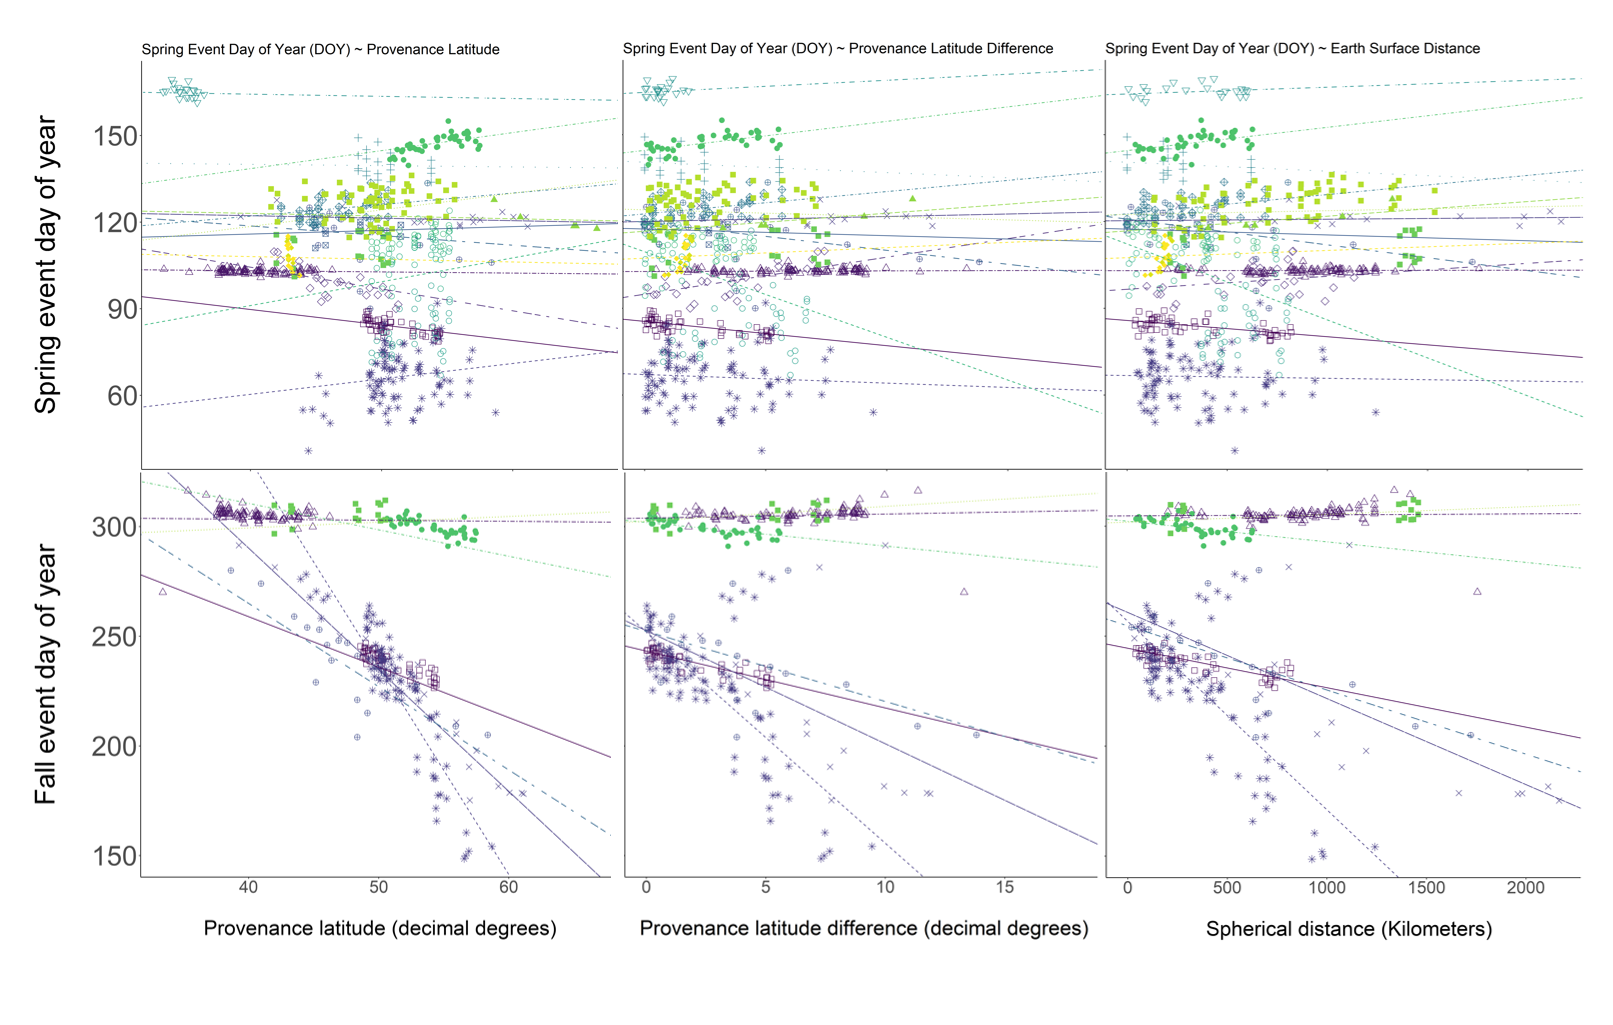
\includegraphics[width=\textwidth]{..//..//localadaptclim/Docs/figure_supp/lat_latdiff_earth_distance.png}
    \caption{Similar results across provenance latitude, absolute value of difference between provenance and garden latitude, and spherical distance}
    \label{figure:lat_distance}
\end{figure}
\todo[inline]{change caption later}

\subsection* {Strong relationship between provenance latitude, MAT, and GDDs}
\todo[inline]{Flagged for Lizzie: I am unsure about how to commment on what we are seeing in this plot. \newline There is a strong relationship between GDDs of each event day recorded and the latitude and MAT, but isn't that self-apparent? }

Placeholder text (Fig. \ref{figure:gdd}).

% all figures will be updated (color, font size, resolution)
\begin{figure}[!h] 
    \centering
 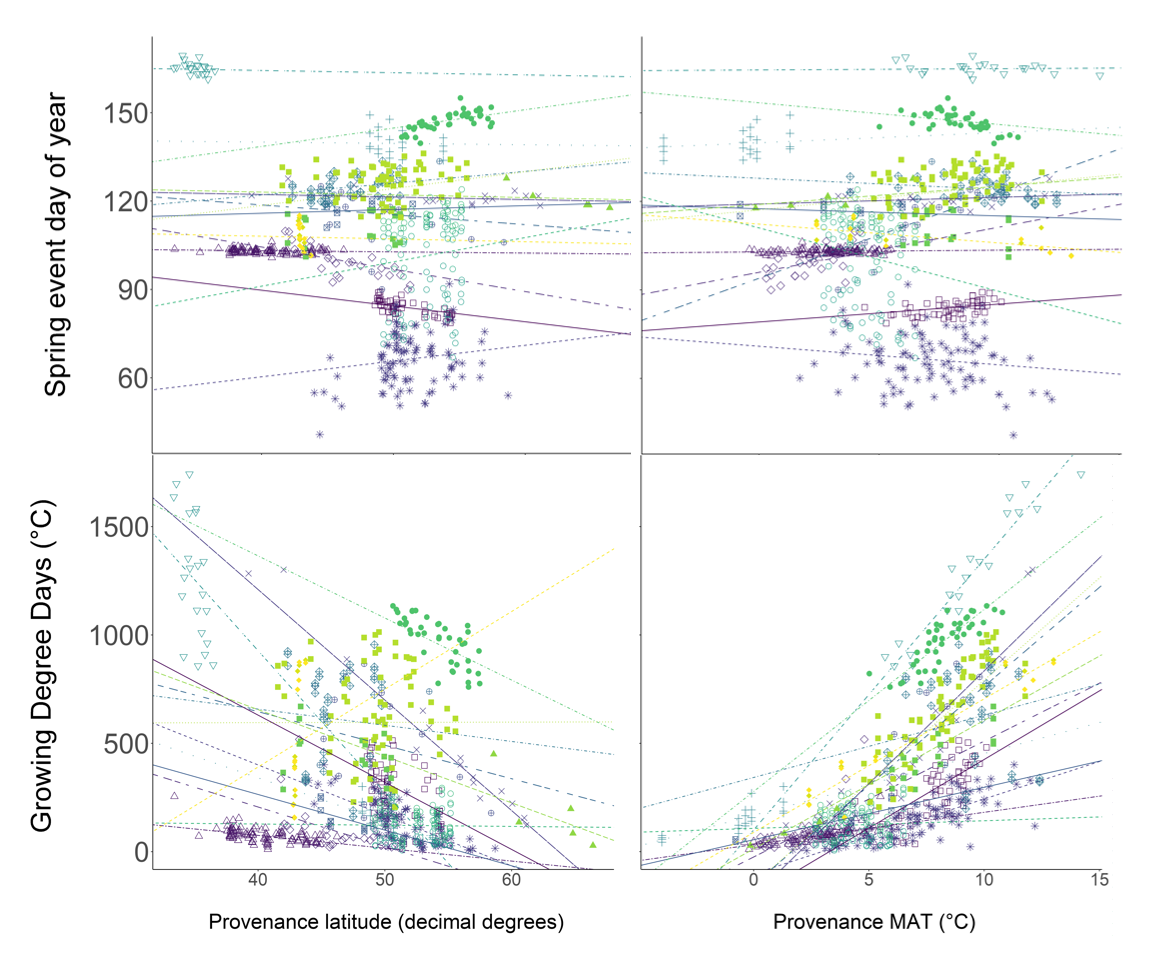
\includegraphics[width=\textwidth]{..//..//localadaptclim/Docs/figure_ms/gdd_ms.png}
    \caption{Growing Degree Days (GDD)on each day of spring event in relation to provenance latitude and MAT, coded by symbol for species and color for garden with linear fits from hierarchical Bayesian models.}
    \label{figure:gdd}
\end{figure}


\section {Don't have a specific sections for these ones yet}

\begin{figure}[!h] 
    \centering
 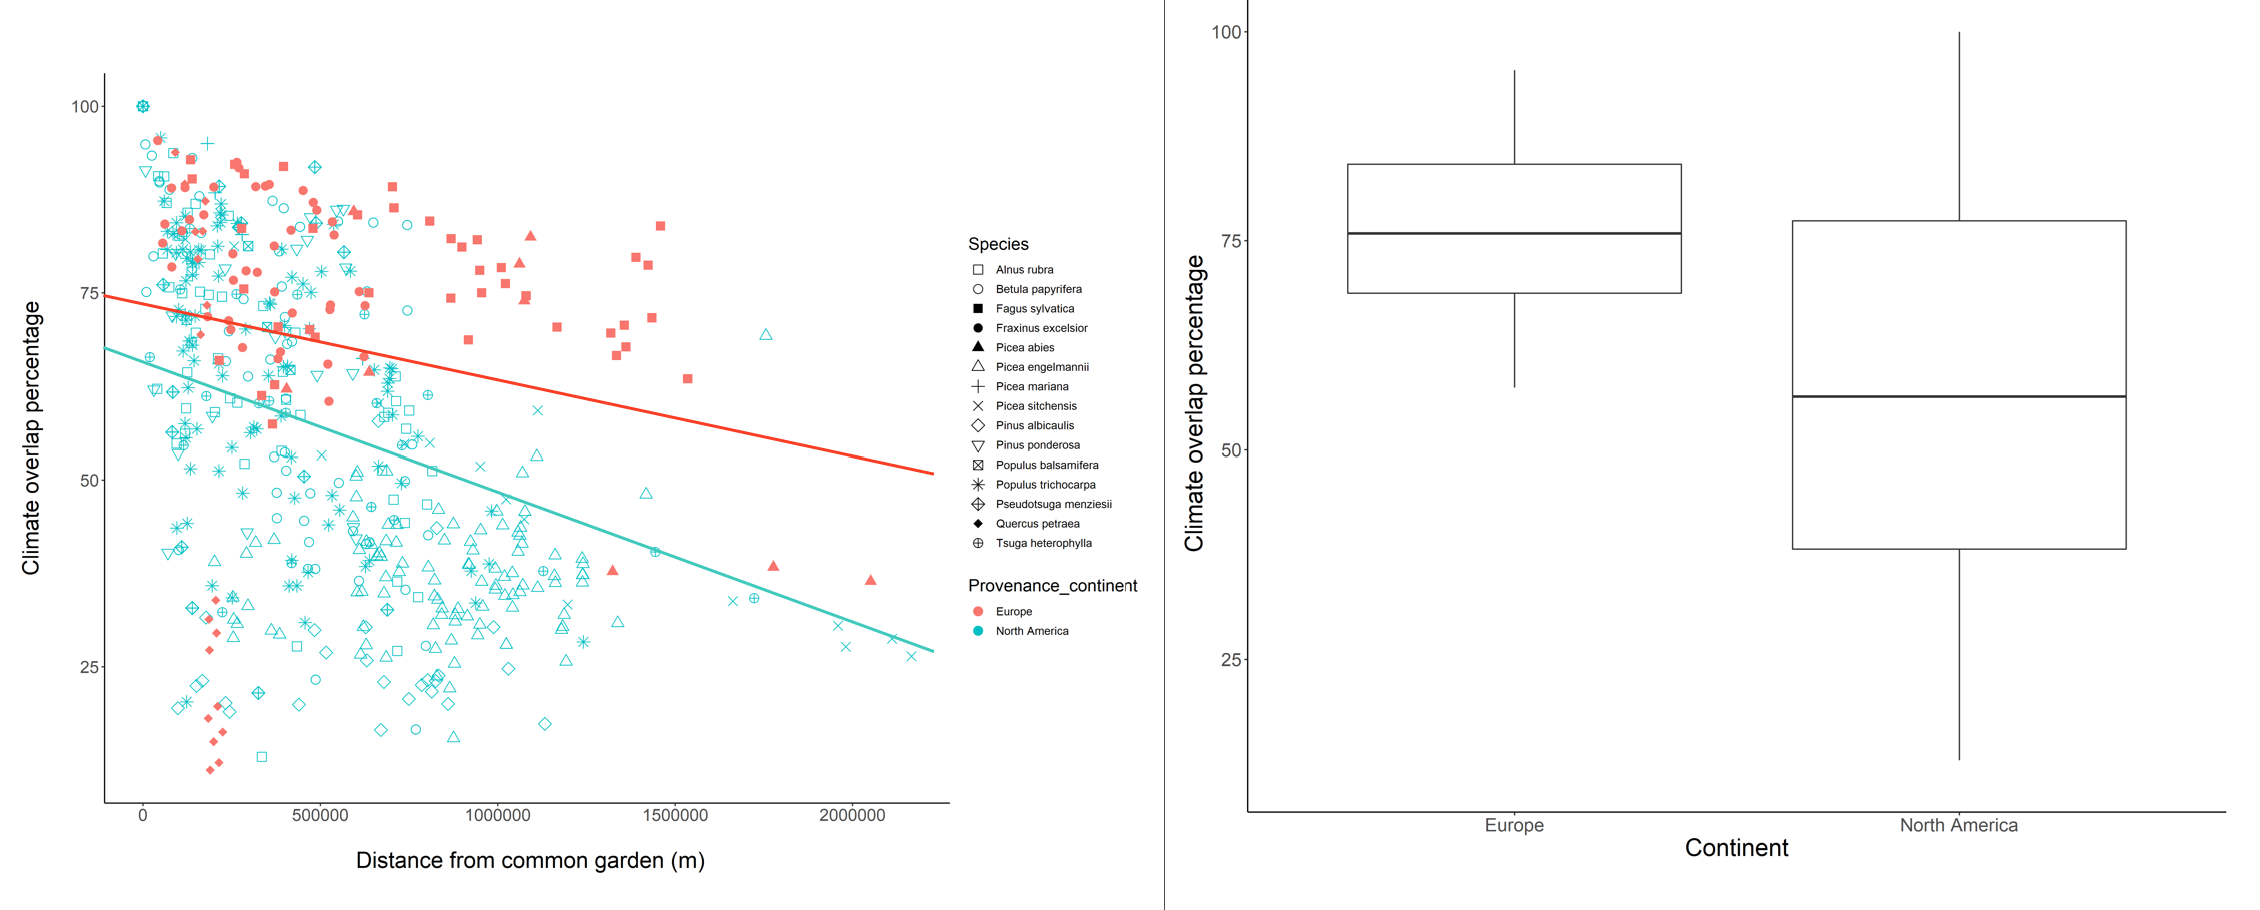
\includegraphics[width=\textwidth]{..//..//localadaptclim/Docs/figure_supp/climate_overlap_continent_comparison.png}
    \caption{The closer a garden is to a provenance, the more overlap in temperature. 
Higher extend of climate overlap in European studies.}
    \label{figure:overlap_continent}
\end{figure}

\begin{figure}[!h] 
    \centering
 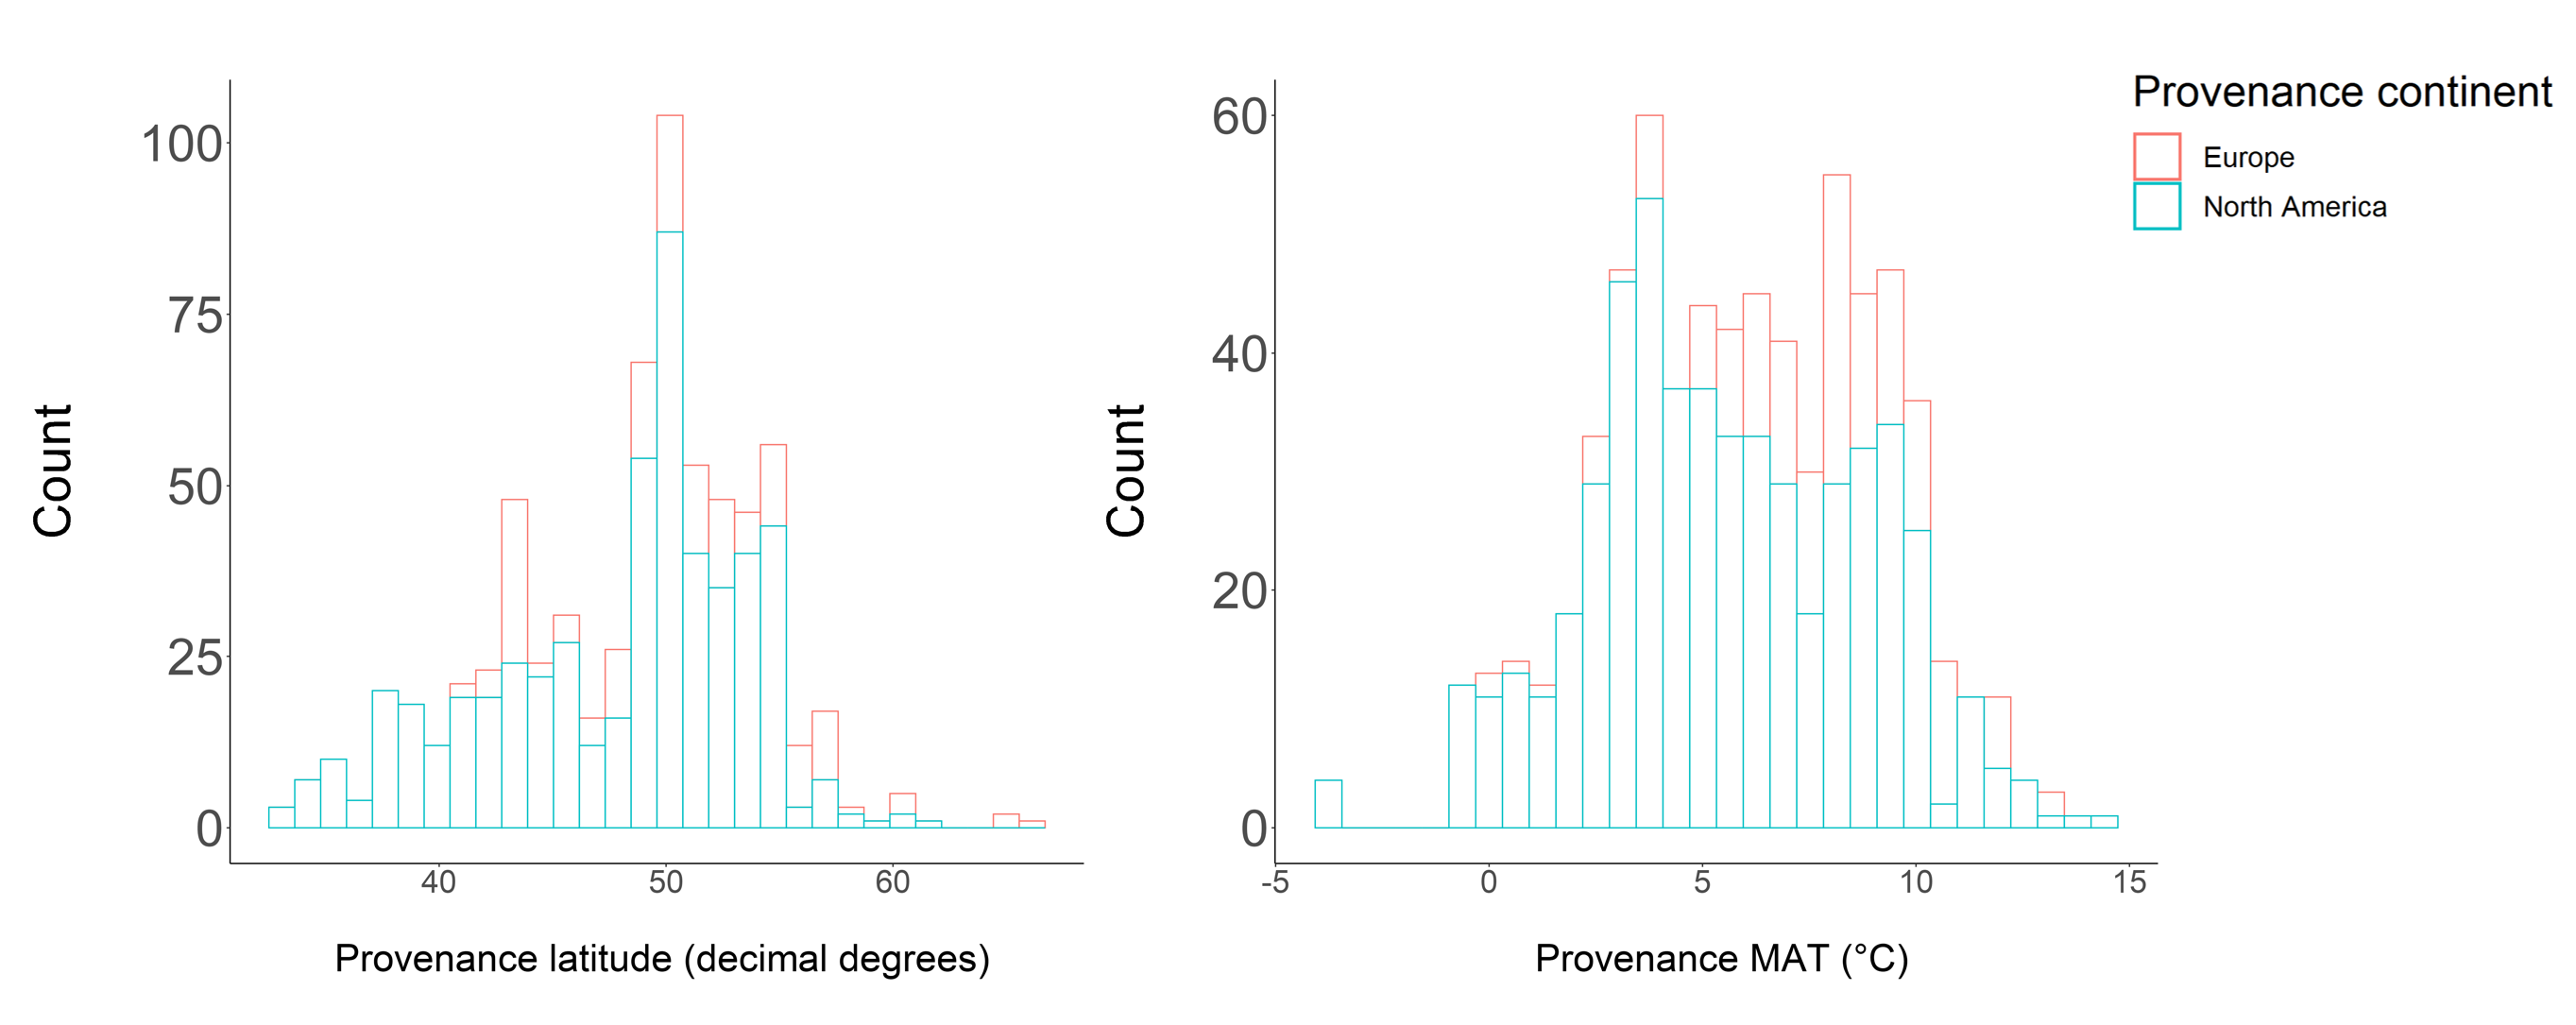
\includegraphics[width=\textwidth]{..//..//localadaptclim/Docs/figure_supp/prov_lat_mat_continent.png}
    \caption{Placeholder.}
    \label{figure:lat_mat_continent}
\end{figure}


\begin{figure}[!h] 
    \centering
 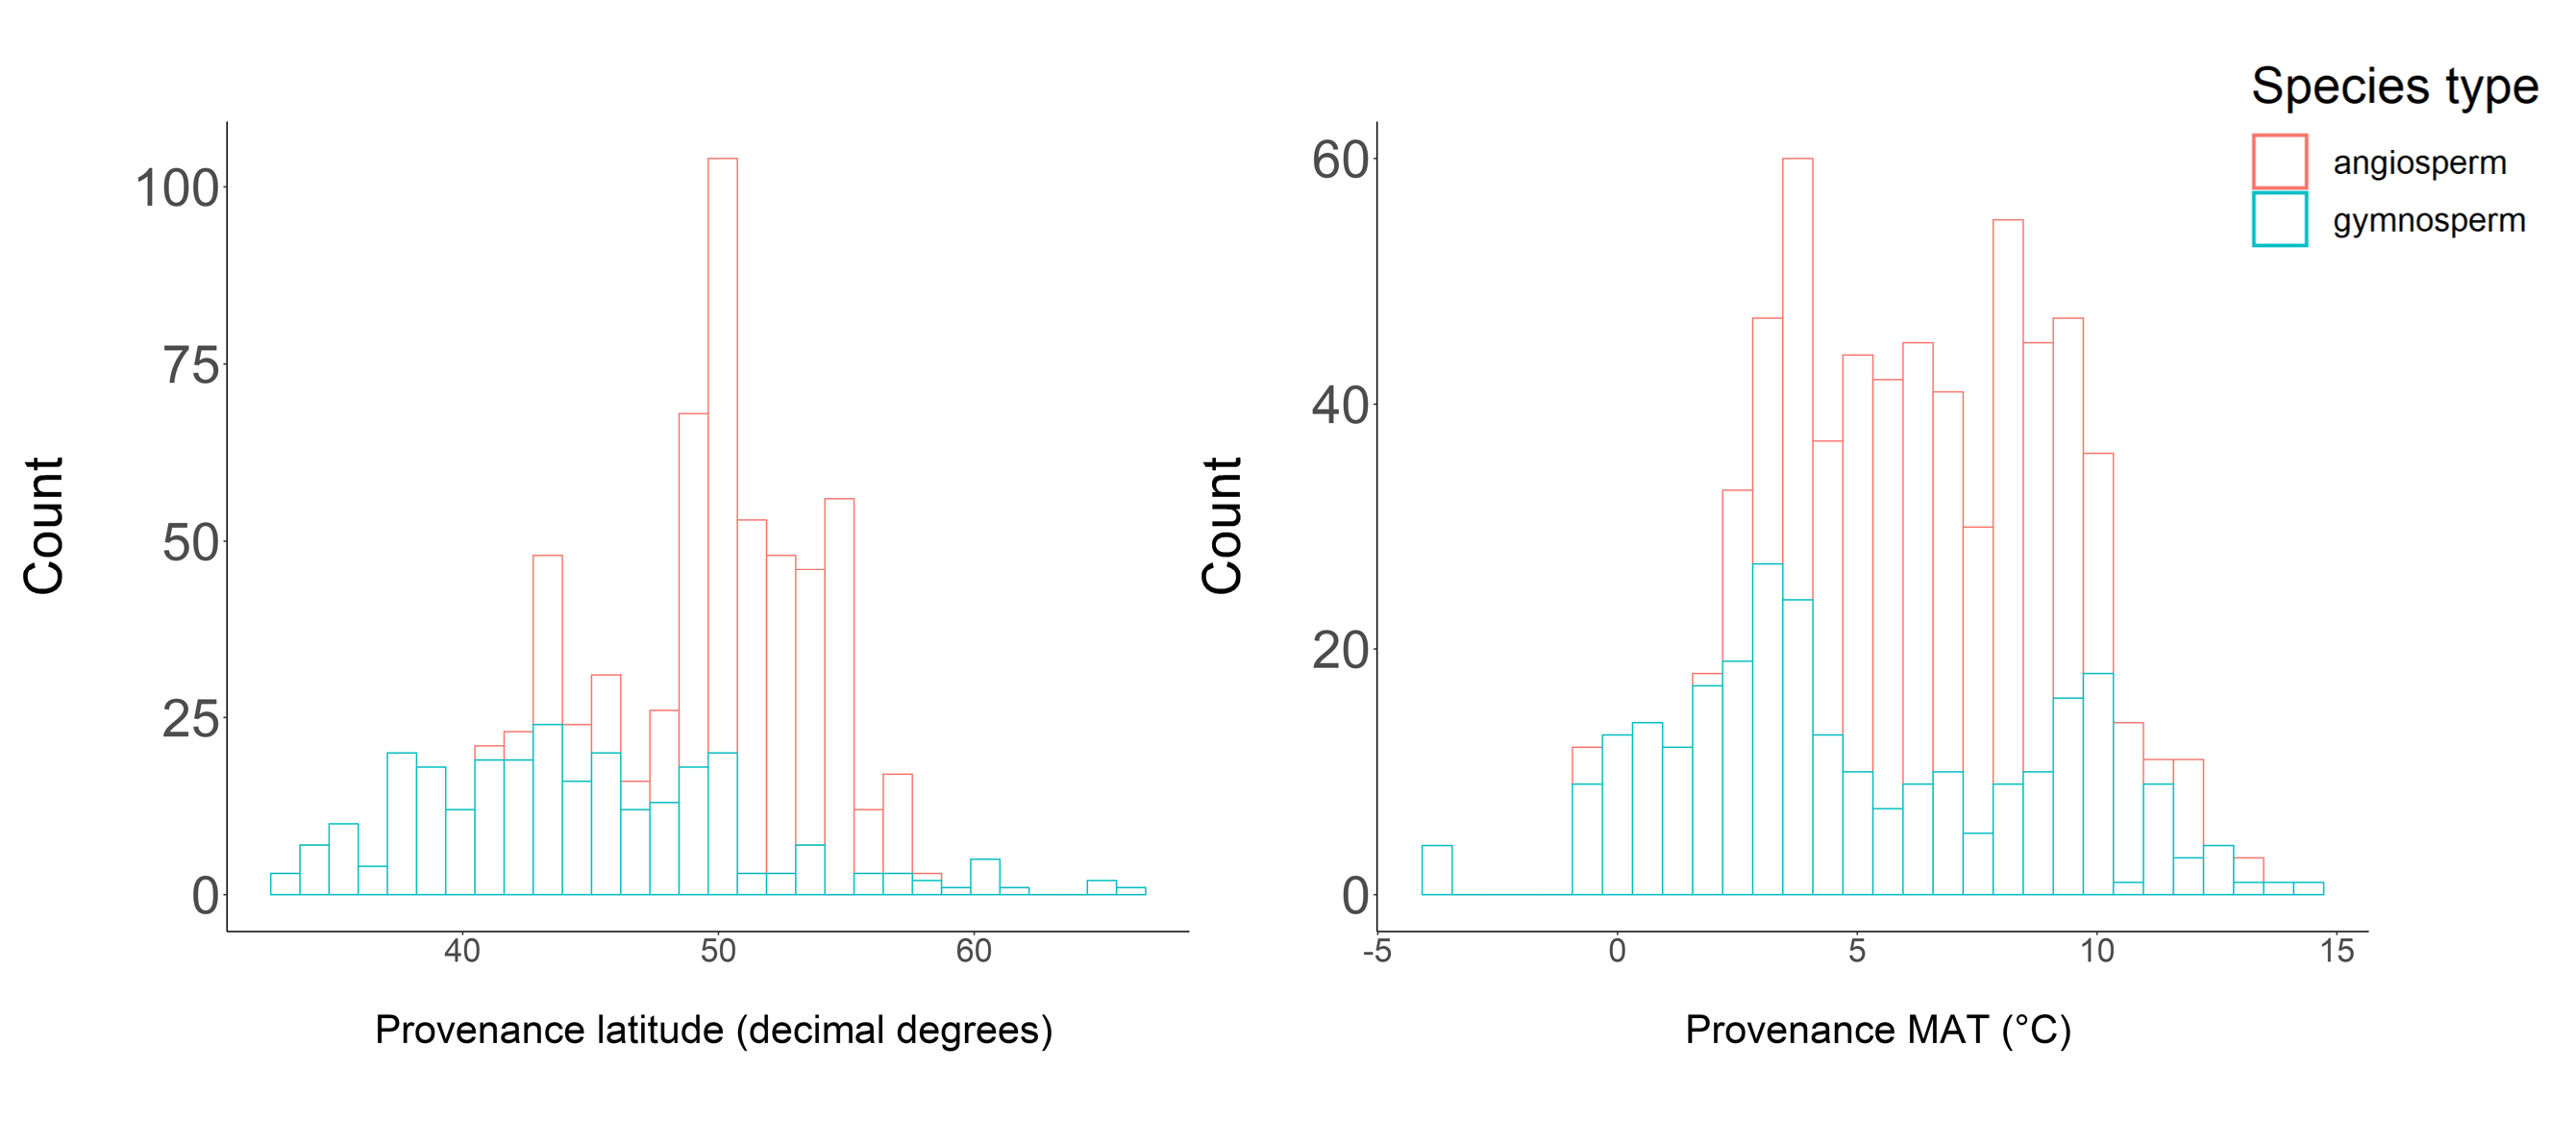
\includegraphics[width=\textwidth]{..//..//localadaptclim/Docs/figure_supp/spp_type_continent.png}
    \caption{Placeholder}
    \label{figure:spp_continent}
\end{figure}

\subsection*{Spring Lat VS. Fall Lat}
\begin{table}
\centering
\caption{Model summary for the relationship between event day of year (DOY)and provenance latitude, fitted by species, in spring (left) and fall (right).}
\todo[inline]{i'm not sure how to word this}
\begin{tabular}[t]{lcc}
\toprule
  & $DOY_{Spring}~(Latitude|Species)$ & $DOY_{Fall}~(Latitude|Species)$\\
\midrule
Intercept & \num{114.219} & \num{316.736}\\
 & {}[\num{100.511}, \num{127.680}] & {}[\num{272.545}, \num{415.373}]\\
Sigma[Species × Intercept,Intercept] & \num{1148.104} & \num{12381.073}\\
 & {}[\num{435.227}, \num{2825.532}] & {}[\num{6176.075}, \num{24554.731}]\\
Sigma[Species × Latitude,Intercept] & \num{-13.454} & \num{-307.256}\\
 & {}[\num{-41.733}, \num{-1.069}] & {}[\num{-621.049}, \num{-122.796}]\\
Sigma[Species × Latitude,Latitude] & \num{0.374} & \num{10.159}\\
 & {}[\num{0.111}, \num{1.030}] & {}[\num{5.266}, \num{33.131}]\\
\midrule
Num.Obs. & \num{671} & \num{349}\\
R2 & \num{0.903} & \num{0.961}\\
R2 Adj. & \num{0.902} & \num{0.960}\\
R2 Marg. & \num{0.000} & \num{0.000}\\
Log.Lik. & \num{-2340.362} & \num{-1217.949}\\
ELPD & \num{-2358.2} & \num{-1231.9}\\
ELPD s.e. & \num{27.8} & \num{22.1}\\
LOOIC & \num{4716.4} & \num{2463.8}\\
LOOIC s.e. & \num{55.6} & \num{44.2}\\
WAIC & \num{4716.2} & \num{2463.3}\\
RMSE & \num{7.87} & \num{8.44}\\
r2.adjusted.marginal & \num{0.902} & \num{0.960}\\
\bottomrule
\end{tabular}
\label{table:model_sf_lat}
\end{table}

\end{document}
